%' Directed acyclic graph (DAG) with arrow text annotations
%'
%' DAG illustrating the partition of subjectivity in a potential mixed-item 
%' IRT models.

\documentclass[12pt,preview,border=0]{standalone}
\usepackage[paperheight=10cm,paperwidth=10cm]{geometry}
\usepackage{graphicx}
\usepackage{amsmath}
\usepackage{kmath,kerkis}
\usepackage{tikz}
\usetikzlibrary{arrows,automata,positioning}

\begin{document} 
\begin{center}

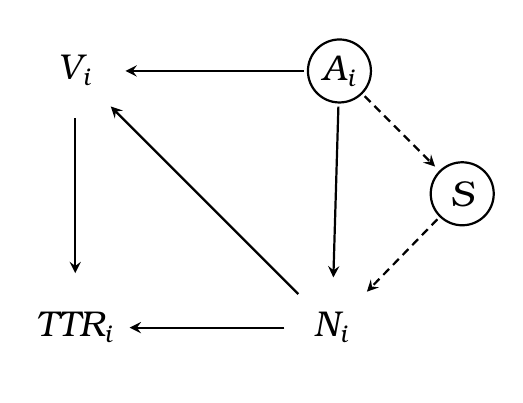
\begin{tikzpicture}[
	> = stealth, % arrow head style
	shorten > = 1pt, % don't touch arrow head to node
	auto,
	node distance = 2cm, % distance between nodes
	thick, % line style
	U/.style={circle, draw=black, inner sep=1.8pt, outer sep=1.5pt, minimum size=8mm, font=\Large},  %draw=black, fill=white
	O/.style={circle, inner sep=1.5pt, outer sep=1.5pt, minimum size=11mm, font=\Large},              %draw=white, fill=white
	]
	
    % Objective items
	% Nodes and their relative positions
	\node[O] (D) {$TTR_i$};
	\node[O] (V) [above = of D] {$V_i$};
    \node[O] (N) [right = of D] {$N_i$};
    \node[U] (A) [right = 2.3 of V] {$A_i$};
    \node[U] (S) [below right = 1.3 of A, opacity=1] {$S$};

	% Paths connecting nodes
    \path[->] (A) edge (V);
    \path[->] (V) edge (D);
	\path[->] (N) edge (D);
    \path[->] (A) edge (N);
    \path[->] (N) edge (V);
    \path[->] (A) edge[densely dashed, opacity=1] (S);
    \path[->] (S) edge[densely dashed, opacity=1] (N);
\end{tikzpicture}

\end{center}\end{document}
